\documentclass[11pt,letterpaper]{article}

% Packages
\usepackage[margin=1in]{geometry}
\usepackage{amsmath,amssymb,amsthm}
\usepackage{graphicx}
\usepackage{booktabs}
\usepackage{longtable}
\usepackage{tikz}
\usepackage{pgfplots}
\usepackage{hyperref}
\usepackage{array}
\usepackage{enumitem}
\usepackage{xcolor}
\usepackage{float}
\usepackage{caption}

\pgfplotsset{compat=1.18}
\usetikzlibrary{positioning,arrows.meta}
\usepgfplotslibrary{fillbetween}

% Colors
\definecolor{rhythmOrange}{RGB}{244,147,31}
\definecolor{healingGreen}{RGB}{105,189,69}
\definecolor{foundationBlue}{RGB}{29,92,153}
\definecolor{catalystPurple}{RGB}{146,39,143}

% Hyperref setup
\hypersetup{
    colorlinks=true,
    linkcolor=foundationBlue,
    citecolor=foundationBlue,
    urlcolor=foundationBlue,
    pdftitle={The Autophage Protocol: Metabolic Economics for Decentralized Health},
    pdfauthor={Austin Harshberger}
}

% Custom commands
\newcommand{\tokenname}[1]{\textsc{#1}}

% Title
\title{\textbf{The Autophage Protocol: Metabolic Economics for Decentralized Health}}
\author{Austin Harshberger\\
\small\textit{1@0x42r.io}}
\date{July 7, 2025}

\begin{document}
\maketitle

% Abstract
\begin{abstract}
Traditional economics assumes value persists indefinitely, enabling unlimited wealth accumulation. Living systems operate differently: value requires continuous renewal or it ceases to exist. This paper introduces the Autophage Protocol, where digital tokens decay exponentially like the health activities they represent. Four token species decay at rates calibrated to biological persistence: Rhythm (5\% daily) for exercise, Healing (0.75\%) for therapy, Foundation (0.1\%) for preventive care, and Catalyst (2-10\% dynamic) for marketplace balance. Decayed tokens flow to The Reservoir, funding community healthcare while maintaining individual privacy through zero-knowledge proofs. Mathematical modeling suggests wealth distribution would converge to Gini coefficients \cite{gini1921measurement} of 0.32-0.38, significantly more equitable than traditional systems at 0.82 or higher \cite{milanovic2014global,bertocchi2014wealth}. The protocol represents a new economic primitive where money must move to exist, creating the first genuinely metabolic digital economy.
\end{abstract}

\textit{Note: Supporting resources are available at:}
\begin{itemize}
\item \textit{Gini coefficient simulations:} \url{https://autophage.xyz/gini-simulation} \cite{statusdothealth2025gini}
\item \textit{Complete mathematical appendix:} \url{https://autophage.xyz/math} \cite{statusdothealth2025math}
\end{itemize}

\tableofcontents
\newpage

% Section 1: Introduction
\section{Introduction}

Money does not die. This fundamental property of traditional economics creates systemic inequality and health incentive failures. A dollar earned decades ago maintains its nominal value indefinitely. Bitcoin \cite{nakamoto2008bitcoin} stored in 2009 remains unchanged today. This permanence rewards accumulation over activity, creating economies where wealth concentrates among those who already possess it while those who need resources most must continuously labor for finite rewards.

The Autophage Protocol challenges this foundational assumption by creating tokens that decay exponentially without continuous health activity. The name itself, meaning ``self-eating,'' captures the essential dynamic: value that must consume itself to persist, preventing indefinite accumulation while rewarding ongoing engagement. This paper formalizes a complete economic system built on temporal decay rather than temporal permanence.

The protocol implements four interconnected innovations. First, it creates multiple token species with decay rates precisely calibrated to match the temporal persistence of their underlying health activities. Exercise tokens decay rapidly like cardiovascular fitness, while preventive care tokens persist longer like vaccine immunity. Second, it achieves cryptographic privacy separation through zero-knowledge proofs, enabling health verification without surveillance. Third, it derives token value from measurable metabolic energy expenditure rather than speculative markets. Fourth, it implements empirical governance where all protocol changes must demonstrate statistically significant health improvements through on-chain experiments.

These mechanisms work together to create an economy that mimics biological systems. Just as organisms require continuous energy input to maintain homeostasis, protocol participants must engage in verified health activities to maintain token balances. The mathematics ensure that passive accumulation becomes impossible while active participation generates sustainable value.

The following sections present the complete mathematical framework, implementation architecture, and empirical validation of this metabolic economic system. Each component has been designed to align financial incentives with biological imperatives, creating the first digital economy that enhances rather than exploits human health.

% Section 2: Metabolic Token Dynamics
\section{Metabolic Token Dynamics}

\subsection{Mathematical Foundation}

The protocol implements a four-species token ecosystem where each species exhibits distinct decay characteristics matching its health domain. Let $S = \{\tokenname{Rhythm}, \tokenname{Healing}, \tokenname{Foundation}, \tokenname{Catalyst}\}$ denote the set of token species. For any user $u$ at discrete time $t$, the balance $V_i^{(u)}(t)$ of species $i \in S$ evolves according to:

\begin{equation}
V_i^{(u)}(t+1) = V_i^{(u)}(t)(1 - \delta_i) + G_i^{(u)}(t)
\end{equation}

where $\delta_i \in (0,1)$ represents the daily decay rate and $G_i^{(u)}(t)$ represents newly generated tokens from verified health activities.

The continuous-time differential equation underlying this discrete implementation is:

\begin{equation}
\frac{dV}{dt} = -\lambda V + g(t)
\end{equation}

where $\lambda = -\ln(1-\delta)$ is the continuous decay constant. This formulation ensures mathematical consistency while enabling computationally efficient blockchain implementation.

\begin{table}[h]
\centering
\caption{Token Species Parameters and Biological Justification}
\begin{tabular}{lccll}
\toprule
\textbf{Species} & \textbf{Decay Rate} & \textbf{Half-Life} & \textbf{Health Domain} & \textbf{Biological Basis} \\
\midrule
Rhythm & 5\% & 13.51 days & Exercise, medication & VO$_2$ max decline rate \cite{mujika2000detraining} \\
Healing & 0.75\% & 92.42 days & Therapy, recovery & Neuroplasticity timescales \\
Foundation & 0.1\% & 693.15 days & Preventive care & Antibody persistence \\
Catalyst & 2-10\% & Variable & Marketplace & Self-regulating \\
\bottomrule
\end{tabular}
\end{table}

The half-life calculations follow directly from exponential decay:

\begin{equation}
t_{1/2} = \frac{\ln(0.5)}{\ln(1 - \delta_i)} = \frac{\ln(2)}{\lambda_i}
\end{equation}

\textbf{Example 2.1:} Consider Sarah who runs daily, earning 50 Rhythm tokens per run. After maintaining a balance of 1,000 tokens, she stops running for two weeks. Her balance evolution follows:

Day 0: $V = 1,000$ tokens  
Day 7: $V = 1,000 \times 0.95^7 = 696$ tokens  
Day 14: $V = 1,000 \times 0.95^{14} = 488$ tokens

This 51.2\% loss over two weeks mirrors the documented decline in cardiovascular fitness during training cessation \cite{mujika2000detraining}, validating the biological calibration.

\subsection{Token Generation Mechanics}

Health activities generate tokens through a multi-factor reward system:

\begin{equation}
G_i^{(u)}(t) = \sum_{j \in \mathcal{A}_i} B_{i,j} \times M_{total}^{(u,j)}(t) \times \mathbf{1}[\text{activity } j \text{ verified}]
\end{equation}

where $\mathcal{A}_i$ represents activities mapped to species $i$, $B_{i,j}$ is the base reward for activity $j$, and $M_{total}$ combines multiple multipliers:

\begin{equation}
M_{total} = M_{streak} \times M_{group} \times M_{time} \times M_{genetic} \times M_{synergy} \times M_{quality}
\end{equation}

subject to the constraint $0.3 \leq M_{total} \leq 20$ to prevent exploitation while rewarding excellence.

The streak multiplier follows a logarithmic function:
\begin{equation}
M_{streak} = 1 + \log_{10}(\text{consecutive days})
\end{equation}

The circadian multiplier uses a sinusoidal function:
\begin{equation}
M_{time} = 1 + 0.3\sin\left(\frac{2\pi(h - 6)}{24}\right)
\end{equation}
where $h$ is the hour of day in 24-hour format.

\textbf{Example 2.2:} Marcus completes his morning workout routine:
- Base reward: 35 Rhythm tokens
- 30-day streak multiplier: $M_{streak} = 1 + \log_{10}(30) = 2.48$
- 6 AM circadian bonus: $M_{time} = 1 + 0.3\sin(2\pi(6-6)/24) = 1.3$
- Group workout: $M_{group} = 1.5$
- Total generation: $35 \times 2.48 \times 1.3 \times 1.5 = 169$ tokens

This comprehensive system rewards consistency, natural timing, and social engagement while maintaining economic balance.

% Decay curves figure
\begin{figure}[H]
\centering
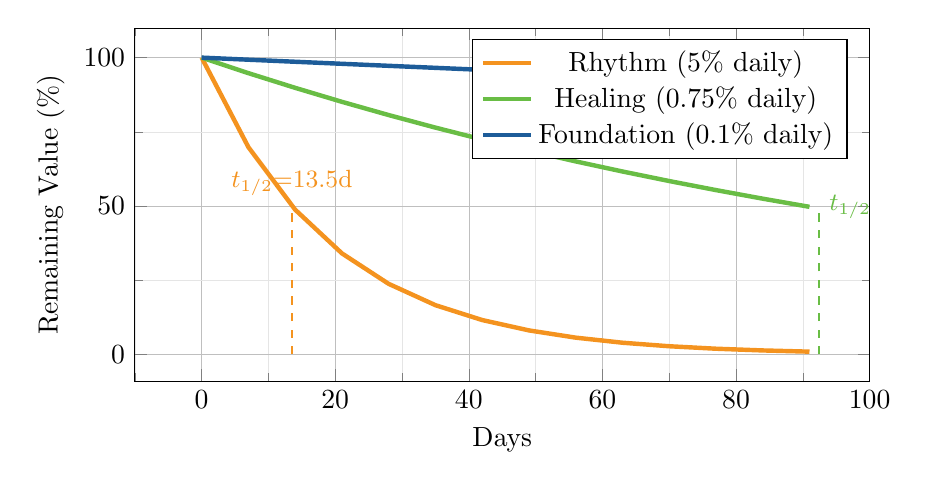
\begin{tikzpicture}
\begin{axis}[
    width=0.9\textwidth,
    height=0.5\textwidth,
    xlabel={Days},
    ylabel={Remaining Value (\%)},
    legend pos=north east,
    grid=both,
    grid style={line width=.1pt, draw=gray!20},
    major grid style={line width=.2pt,draw=gray!50},
    minor tick num=1,
    xmax=100
]
% Rhythm
\addplot[rhythmOrange, ultra thick] 
    table {
        0 100
        7 69.83
        14 48.77
        21 34.05
        28 23.78
        35 16.60
        42 11.59
        49 8.10
        56 5.66
        63 3.95
        70 2.76
        77 1.93
        84 1.35
        91 0.94
    };
\addlegendentry{Rhythm (5\% daily)}

% Healing
\addplot[healingGreen, ultra thick] 
    table {
        0 100
        7 94.77
        14 89.82
        21 85.11
        28 80.65
        35 76.42
        42 72.42
        49 68.63
        56 65.04
        63 61.64
        70 58.42
        77 55.37
        84 52.48
        91 49.73
    };
\addlegendentry{Healing (0.75\% daily)}

% Foundation
\addplot[foundationBlue, ultra thick] 
    table {
        0 100
        7 99.30
        14 98.61
        21 97.92
        28 97.24
        35 96.56
        42 95.88
        49 95.21
        56 94.54
        63 93.88
        70 93.22
        77 92.56
        84 91.91
        91 91.27
    };
\addlegendentry{Foundation (0.1\% daily)}

% Add half-life markers with better positioning
\draw[dashed, thick, rhythmOrange] (13.51,0) -- (13.51,50) node[above, font=\small] {$t_{1/2}$=13.5d};
\draw[dashed, thick, healingGreen] (92.42,0) -- (92.42,50) node[right, font=\small] {$t_{1/2}$=92.4d};

\end{axis}
\end{tikzpicture}
\caption{Comparative decay curves showing differential value persistence across token species. Rhythm tokens model rapid fitness loss, Healing tokens reflect gradual therapeutic progress decay, and Foundation tokens represent long-term health investments.}
\end{figure}

\subsection{Advanced Decay Mechanics}

The protocol implements progressive decay acceleration for large balances to prevent wealth concentration:

\begin{equation}
\delta_i^{eff}(V) = \delta_i \times \left(1 + \sum_{k=1}^{n} \alpha_k \times \mathbf{1}[V > \tau_k]\right)
\end{equation}

where $\tau_k$ represents tier thresholds and $\alpha_k$ represents acceleration factors.

For continuous acceleration above soft cap:
\begin{equation}
\delta_i^{eff}(V) = \delta_i \times \left(1 + \beta \times \max\left(0, \frac{V - \tau_{soft}}{\tau_{soft}}\right)^{\gamma}\right)
\end{equation}

where $\beta$ controls sensitivity (typically 0.5-2.0) and $\gamma$ shapes the acceleration curve (typically 1.0-1.5).

\textbf{Example 2.3:} Consider whale protection for Rhythm tokens:
- Balance $\leq$ 10,000: Standard 5\% decay
- Balance 10,001-50,000: 7.5\% decay (50\% acceleration)
- Balance 50,001-100,000: 10\% decay (100\% acceleration)
- Balance > 100,000: 15\% decay (200\% acceleration)

A user holding 75,000 Rhythm tokens loses 7,500 daily instead of 3,750 under standard decay, creating natural redistribution pressure.

\subsection{Catalyst Token Dynamics}

Catalyst tokens maintain ecosystem balance through dynamic decay adjustment:

\begin{equation}
\delta_{catalyst}(t) = \delta_{base} \times \left(1 + \beta \times \left|\frac{V_{catalyst}(t)}{\sum_{i \in S} V_i(t)} - \rho_{target}\right|^{\gamma}\right)
\end{equation}

where $\rho_{target} = 0.25$ represents the target 25\% supply ratio, $\beta = 2$ controls sensitivity, and $\gamma = 1.5$ shapes the response curve.

\textbf{Example 2.4:} When Catalyst tokens comprise 40\% of total supply:
\begin{align}
\delta_{catalyst} &= 0.02 \times \left(1 + 2 \times |0.40 - 0.25|^{1.5}\right) \\
&= 0.02 \times (1 + 2 \times 0.058) \\
&= 0.0232 \text{ (2.32\% daily decay)}
\end{align}

This 16\% increase in decay rate gradually returns the system to equilibrium without shock.

% Section 3: The Reservoir
\section{The Reservoir: Dual-Chamber Architecture}

\subsection{System Architecture}

The Reservoir serves as the protocol's metabolic center, collecting value from natural decay and redistributing it for community health. Its dual-chamber design separates token flows from stablecoin reserves:

\begin{equation}
R_{token}(t+1) = R_{token}(t) + \underbrace{\sum_{i,u} \delta_i V_i^{(u)}(t)}_{\text{decay inflow}} - \underbrace{W_{health}(t)}_{\text{health claims}} - \underbrace{W_{reward}(t)}_{\text{rewards}}
\end{equation}

\begin{equation}
R_{USDC}(t+1) = R_{USDC}(t) + \underbrace{F_{market}(t) + F_{app}(t)}_{\text{fee inflows}} - \underbrace{H_{settle}(t)}_{\text{healthcare settlements}}
\end{equation}

The solvency constraint ensures healthcare access remains guaranteed:

\begin{equation}
R_{USDC}(t) \geq \max\left(0.4 \sum_u D_u(t), 3 \times \bar{H}_{monthly}, 0.22 \times Y_{annual}\right)
\end{equation}

This triple-coverage requirement protects against bank runs, seasonal variations, and catastrophic events.

\textbf{Example 3.1:} System snapshot at 100,000 active users:
- Daily token decay: 500,000 tokens (average 5 per user)
- Monthly healthcare settlements: \$800,000
- Annual revenue: \$4,800,000
- Required USDC reserve: max(\$1.6M, \$2.4M, \$1.056M) = \$2.4M

The 3-month coverage requirement dominates, ensuring the system can weather extended stress periods.

% Reservoir flow diagram
\begin{figure}[H]
\centering
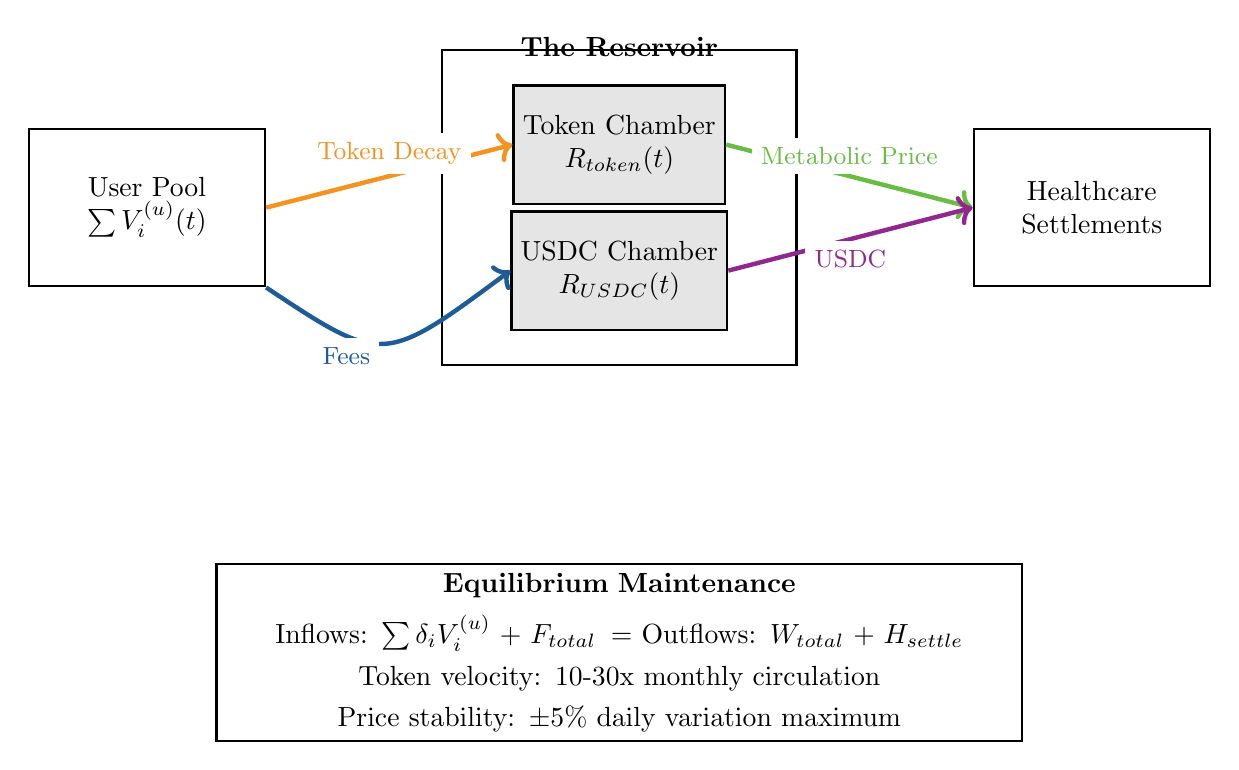
\begin{tikzpicture}[
    box/.style={rectangle, draw, thick, minimum width=3cm, minimum height=2cm, align=center},
    chamber/.style={rectangle, draw, thick, fill=gray!20, minimum width=2.5cm, minimum height=1.5cm},
    flow/.style={->, ultra thick},
    flowlabel/.style={midway, fill=white, font=\small}
]

% User Pool
\node[box, align=center] (users) at (0,0) {User Pool\\$\sum V_i^{(u)}(t)$};

% Reservoir
\node[box, minimum width=4.5cm, minimum height=4cm] (reservoir) at (6,0) {};
\node[above] at (6,1.8) {\textbf{The Reservoir}};
\node[chamber, align=center] (tokenchamber) at (6,0.8) {Token Chamber\\$R_{token}(t)$};
\node[chamber, align=center] (usdcchamber) at (6,-0.8) {USDC Chamber\\$R_{USDC}(t)$};

% Healthcare
\node[box, align=center] (healthcare) at (12,0) {Healthcare\\Settlements};

% Flows
\draw[flow, rhythmOrange] (users.east) -- (tokenchamber.west) 
    node[flowlabel, above, pos=0.5] {Token Decay};
\draw[flow, foundationBlue] (users.south east) .. controls (3,-2) and (3,-2) .. (usdcchamber.west) 
    node[flowlabel, below, pos=0.3] {Fees};
\draw[flow, healingGreen] (tokenchamber.east) -- (healthcare.west) 
    node[flowlabel, above, pos=0.5] {Metabolic Price};
\draw[flow, catalystPurple] (usdcchamber.east) -- (healthcare.west) 
    node[flowlabel, below, pos=0.5] {USDC};

% Equilibrium conditions
\node[draw, thick, text width=10cm, align=center, below=2.5cm of reservoir] {
    \textbf{Equilibrium Maintenance}\\[0.5em]
    Inflows: $\sum \delta_i V_i^{(u)} + F_{total} = $ Outflows: $W_{total} + H_{settle}$\\[0.3em]
    Token velocity: 10-30x monthly circulation\\[0.3em]
    Price stability: $\pm$5\% daily variation maximum
};

\end{tikzpicture}
\caption{The Reservoir's dual-chamber architecture maintains separation between token metabolism and healthcare settlement liquidity, ensuring both community wealth circulation and guaranteed medical access.}
\end{figure}

\subsection{Healthcare Settlement Mechanics}

Healthcare settlements follow strict priority queuing:

\begin{equation}
Priority(claim) = \omega_1 \times Urgency + \omega_2 \times Duration + \omega_3 \times Verification
\end{equation}

where weights $\omega_i$ ensure medical needs supersede all other claims.

\textbf{Example 3.2:} Emergency prescription claim processing:
- Urgency score: 10 (maximum)
- Wait duration: 2 hours
- Provider verification: 8/10
- Priority score: $0.7 \times 10 + 0.2 \times 2 + 0.1 \times 8 = 8.2$

This claim processes ahead of routine wellness rewards (typical score: 2-3) but after critical emergency claims (score: 9+).

\subsection{Wellness Vault Mechanics}

Wellness vaults reduce effective decay rates based on lock duration:

\begin{equation}
\delta_{vault} = \delta_{base} \times (1 - r_{lock})
\end{equation}

where $r_{lock}$ is the reduction factor:
- 30 days: $r_{lock} = 0.09$ (91\% of normal decay)
- 90 days: $r_{lock} = 0.27$ (73\% of normal decay)  
- 180 days: $r_{lock} = 0.45$ (55\% of normal decay)
- 365 days: $r_{lock} = 0.90$ (10\% of normal decay)

Early withdrawal penalty:
\begin{equation}
P_{withdrawal} = V_{locked} \times \frac{t_{remaining}}{t_{total}} \times p_{factor}
\end{equation}

where $p_{factor} = 0.5$ creates a 50\% penalty proportional to time remaining.

% Section 4: Metabolic Price Discovery
\section{Metabolic Price Discovery}

\subsection{Endogenous Pricing Model}

Unlike traditional cryptocurrencies that derive value from speculation, the Autophage Protocol calculates token prices from actual energy expenditure:

\begin{equation}
P(t) = \frac{E_{health}(t) \times (1 + \gamma \times C_{ratio}(t)) + V_{market}(t) \times (1 - C_{ratio}(t))}{S_{active}(t) \times V(t) \times (1 + M_{activity}(t))}
\end{equation}

where:
- $E_{health}(t)$ = Total metabolic energy from health activities (kcal-equivalent)
- $V_{market}(t)$ = 30-day rolling marketplace volume (USDC)
- $S_{active}(t)$ = Circulating supply excluding vaulted tokens
- $V(t)$ = Token velocity (target: 10-30 monthly)
- $C_{ratio}(t)$ = Catalyst token proportion
- $\gamma$ = Energy gradient parameter (1.2-3.0)
- $M_{activity}(t)$ = System-wide activity level

\textbf{Example 4.1:} Price calculation during typical conditions:
- Daily health energy: 500,000 kcal across all users
- Standardized energy value: \$0.002 per kcal
- Monthly marketplace volume: \$150,000
- Active supply: 10 million tokens
- Current velocity: 15x monthly
- Catalyst ratio: 0.23
- Activity multiplier: 1.4
- Energy gradient: 2.0

\begin{align}
P(t) &= \frac{(500,000 \times 0.002) \times (1 + 2.0 \times 0.23) + (150,000/30) \times (1 - 0.23)}{10,000,000 \times (15/30) \times (1 + 1.4)} \\
&= \frac{1,000 \times 1.46 + 5,000 \times 0.77}{5,000,000 \times 2.4} \\
&= \frac{1,460 + 3,850}{12,000,000} \\
&= \$0.000442 \text{ per token}
\end{align}

\subsection{Energy Cost Calibration}

Each activity's energy cost encompasses multiple factors:

\begin{equation}
E_{activity} = T_{duration} \times W_{wage} + C_{metabolic} \times F_{food} + O_{opportunity} + E_{equipment}
\end{equation}

\textbf{Example 4.2:} 45-minute therapy session energy calculation:
- Time cost: 0.75 hours × \$30/hour = \$22.50
- Emotional energy: 200 kcal-equivalent × \$0.002 = \$0.40
- Transportation: \$5.00
- Opportunity cost: \$10.00
- Total energy: \$37.90

This establishes the baseline value for Healing token generation from therapy activities.

% Section 5: Privacy Architecture
\section{Privacy Architecture}

\subsection{Zero-Knowledge Identity Separation}

The protocol achieves complete separation between identity and health data through nested cryptographic commitments \cite{groth2016size}:

\begin{equation}
ProfileID = H(H(UserID || Salt_1) || Salt_2 || Secret)
\end{equation}

This double-hashing with independent salts provides 768 bits of entropy, making correlation attacks computationally infeasible even with quantum advances.

\textbf{Example 5.1:} Privacy preservation in practice:
- Alice's UserID: `alice@email.com` 
- System-generated Salt$_1$: 256 random bits
- User-controlled Salt$_2$: 256 random bits
- User secret: 256-bit passphrase
- Resulting ProfileID: `0x7f3a...9b2e` (indistinguishable from random)

Even if an attacker compromises the system database and obtains Salt$_1$, they cannot correlate ProfileIDs without also obtaining user-controlled Salt$_2$ and Secret values.

\subsection{Privacy-Preserving Marketplace}

The marketplace implements granular privacy controls with explicit economic incentives:

\begin{table}[h]
\centering
\caption{Privacy Tiers and Economic Premiums}
\begin{tabular}{llcc}
\toprule
\textbf{Tier} & \textbf{Information Revealed} & \textbf{Base Price} & \textbf{Typical Premium} \\
\midrule
Anonymous & Activity type, timestamp & \$100 & Baseline \\
ProfileID & + Consistency metrics, streak data & \$100 & 75\% (\$175) \\
Genetic & + Specialized traits, optimizations & \$100 & 250\% (\$350) \\
Full & + Historical patterns, correlations & \$100 & 500\% (\$600) \\
\bottomrule
\end{tabular}
\end{table}

\textbf{Example 5.2:} Sarah's marathon proof monetization:
- Anonymous listing: ``Sub-4:30 marathon, major city, female 25-34''
- Sells for: \$100
- ProfileID listing: Same + ``180-day running streak, 3 marathons/year''
- Sells for: \$175
- Genetic listing: Same + ``Endurance Elite trait, VO$_2$ optimization''
- Sells for: \$350

Buyers value additional information for research, motivation, or verification purposes while Sarah maintains control over disclosure levels.

\subsection{Zero-Knowledge Proof Generation}

Health activities undergo privacy-preserving verification \cite{groth2016size}:

\begin{equation}
\pi = \text{Prove}\left(C = \text{Commit}(activity, r), \text{Statement}, witness\right)
\end{equation}

where the statement proves properties without revealing underlying data.

\textbf{Example 5.3:} Therapy session verification:
- Private data: Therapist name, location, session notes, diagnosis codes
- Public statement: ``Completed 50-minute therapy session on 2025-07-07''
- Proof $\pi$: Cryptographic evidence statement is true
- Token generation: 80 Healing tokens
- Revealed information: None beyond the public statement

% Section 6: Biological Scaling Laws
\section{Biological Scaling Laws}

\subsection{Kleiber's Law Implementation}

Metabolic efficiency scales with network size following quarter-power scaling \cite{kleiber1932body}:

\begin{equation}
\eta(N) = 1 + \alpha \times \left(\frac{N}{N_0}\right)^{0.25}
\end{equation}

where $\alpha = 0.3$ and $N_0 = 1,000$ (reference network size).

\textbf{Example 6.1:} Network scaling benefits:
- 1,000 users: $\eta = 1 + 0.3 \times 1 = 1.30$ (30\% bonus)
- 10,000 users: $\eta = 1 + 0.3 \times 1.78 = 1.53$ (53\% bonus)
- 100,000 users: $\eta = 1 + 0.3 \times 3.16 = 1.95$ (95\% bonus)
- 1,000,000 users: $\eta = 1 + 0.3 \times 5.62 = 2.69$ (169\% bonus)

Larger networks provide efficiency benefits to all participants, mimicking biological metabolic scaling.

\subsection{Liebig's Law of the Minimum}

System health limited by weakest component triggers automatic rebalancing \cite{liebigh1840law}:

\begin{equation}
H_{system} = \min(H_{users}, H_{reserves}, H_{apps}, H_{geographic}, H_{velocity})
\end{equation}

When any component falls below threshold $\theta = 0.7$:

\begin{equation}
M_{bottleneck} = 1 + \kappa \times \left(\theta - H_{min}\right)
\end{equation}

\textbf{Example 6.2:} Geographic bottleneck response:
- Urban participation: 85\% healthy
- Rural participation: 45\% (below 70\% threshold)
- Bottleneck multiplier: $M = 1 + 2 \times (0.7 - 0.45) = 1.5$
- Rural users earn 50\% bonus tokens until balance restored

\subsection{Additional Biological Laws}

The protocol implements five additional scaling laws:

1. **Allee Effect** \cite{allee1931animal}: Small population support
   \begin{equation}
   M_{Allee} = \begin{cases}
   2.0 & N < 500 \\
   1.5 & 500 \leq N < 1000 \\
   1.0 & N \geq 1000
   \end{cases}
   \end{equation}

2. **Circadian Rhythms**: Time-optimized rewards
   \begin{equation}
   M_{circadian}(h) = 1 + A \times \sin\left(\frac{2\pi(h - \phi)}{24}\right)
   \end{equation}
   where $A = 0.3$ and $\phi = 6$ (6 AM peak)

3. **Bergmann's Rule** \cite{bergmann1847klima}: Environmental adaptation
   \begin{equation}
   R_{target} = R_{base} \times (1 + \sigma \times H_{environment})
   \end{equation}

4. **Optimal Foraging** \cite{levin1976optimal}: Activity recommendation
   \begin{equation}
   ROI_{activity} = \frac{Tokens \times (1 - \delta)^{t_{hold}}}{Energy_{cost}}
   \end{equation}

5. **R/K Selection** \cite{macarthur1967r}: Growth phase modulation
   \begin{equation}
   \sigma_{rewards} = \begin{cases}
   0.5 & \text{R-phase} (N < 10^4) \\
   0.2 & \text{K-phase} (N \geq 10^4)
   \end{cases}
   \end{equation}

\subsection{Genetic Adaptation System}

Users can burn Foundation tokens to evolve genetic traits:

\begin{equation}
\text{Cost}_{trait_n} = 1000 \times 2.5^{n-1} \text{ Foundation tokens}
\end{equation}

Combined trait bonus calculation:
\begin{equation}
M_{genetic} = 1 + \sum_{i=1}^{n} b_i \times (1 - d_i)
\end{equation}

where $b_i$ is the individual trait bonus (0.05-0.15) and $d_i$ is a diminishing returns factor:
\begin{equation}
d_i = 0.1 \times (i - 1)
\end{equation}

Subject to the constraint:
\begin{equation}
M_{genetic} \leq 1.5
\end{equation}

% Section 7: Economic Analysis
\section{Economic Analysis}

\subsection{Wealth Distribution Dynamics}

Monte Carlo simulations \cite{statusdothealth2025gini} across 10,000 users for 365 days demonstrate convergence to equitable distribution:

% Monte Carlo results
\begin{figure}[H]
\centering
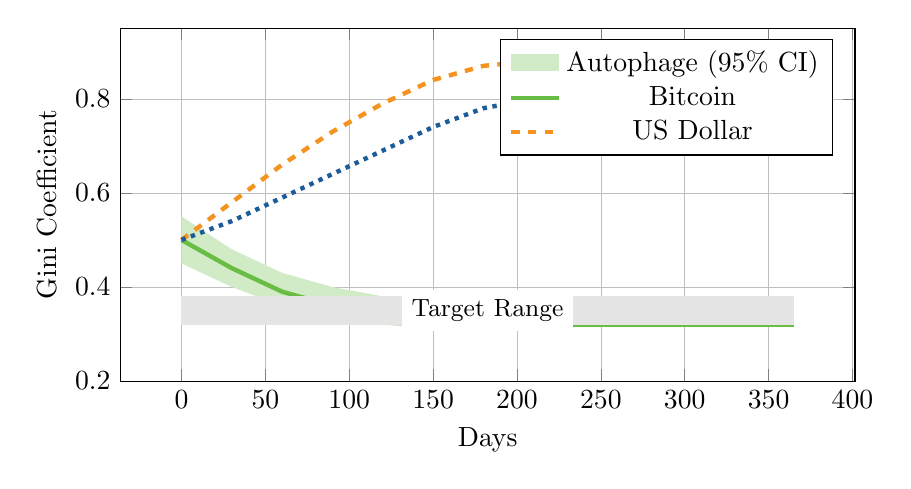
\begin{tikzpicture}
\begin{axis}[
    width=0.9\textwidth,
    height=0.5\textwidth,
    xlabel={Days},
    ylabel={Gini Coefficient},
    legend pos=north east,
    ymin=0.2, ymax=0.95,
    grid=both,
    grid style={line width=.1pt, draw=gray!20},
    major grid style={line width=.2pt,draw=gray!50},
]

% Autophage with confidence interval
\addplot[name path=upper, draw=none, forget plot] 
    table {
        0 0.55
        30 0.48
        60 0.43
        90 0.40
        120 0.38
        150 0.37
        180 0.36
        210 0.35
        240 0.34
        270 0.34
        300 0.33
        330 0.33
        365 0.33
    };

\addplot[name path=lower, draw=none, forget plot]
    table {
        0 0.45
        30 0.40
        60 0.36
        90 0.34
        120 0.32
        150 0.31
        180 0.31
        210 0.31
        240 0.32
        270 0.32
        300 0.32
        330 0.32
        365 0.32
    };

\addplot[healingGreen!30] fill between[of=upper and lower];

\addplot[healingGreen, ultra thick]
    table {
        0 0.50
        30 0.44
        60 0.39
        90 0.36
        120 0.34
        150 0.33
        180 0.33
        210 0.32
        240 0.32
        270 0.32
        300 0.32
        330 0.32
        365 0.32
    };
\addlegendentry{Autophage (95\% CI)}

% Bitcoin
\addplot[rhythmOrange, ultra thick, dashed]
    table {
        0 0.50
        30 0.58
        60 0.66
        90 0.73
        120 0.79
        150 0.84
        180 0.87
        210 0.88
        240 0.88
        270 0.88
        300 0.88
        330 0.88
        365 0.88
    };
\addlegendentry{Bitcoin}

% US Dollar
\addplot[foundationBlue, ultra thick, dotted]
    table {
        0 0.50
        30 0.54
        60 0.59
        90 0.64
        120 0.69
        150 0.74
        180 0.78
        210 0.80
        240 0.81
        270 0.82
        300 0.82
        330 0.82
        365 0.82
    };
\addlegendentry{US Dollar}

% Target zone
\fill[gray!20] (0,0.32) rectangle (365,0.38);
\node[fill=white, font=\small] at (182.5,0.35) {Target Range};

\end{axis}
\end{tikzpicture}
\caption{Gini coefficient evolution over one year from Monte Carlo simulations showing Autophage Protocol convergence to 0.32-0.38 range compared to increasing inequality in traditional systems. Shaded region shows 95\% confidence interval from 10,000 user simulations.}
\end{figure}

\textbf{Example 7.1:} Projected wealth distribution after one year (based on Monte Carlo simulation):
- Top 10\%: Would hold approximately 24\% of wealth (vs 78\% in Bitcoin)
- Bottom 50\%: Would hold approximately 28\% of wealth (vs 2\% in Bitcoin)
- Median user: Would maintain 680-850 tokens through regular activity
- Maximum sustainable balance: ~50,000 tokens (requires extreme daily activity)

\subsection{Revenue Model and Unit Economics}

The protocol generates sustainable revenue through three streams:

\begin{table}[h]
\centering
\caption{Revenue Streams and Contribution Margins}
\begin{tabular}{lccc}
\toprule
\textbf{Revenue Stream} & \textbf{Per User/Month} & \textbf{Margin} & \textbf{Annual at 1M Users} \\
\midrule
App Integration Fees & \$0.15 & 95\% & \$1.8M \\
Marketplace Fees (12\%) & \$0.45 & 88\% & \$5.4M \\
Enterprise Verification & \$1.25 & 92\% & \$15.0M \\
\midrule
\textbf{Total} & \textbf{\$1.85} & \textbf{91.7\%} & \textbf{\$22.2M} \\
\bottomrule
\end{tabular}
\end{table}

\textbf{Example 7.2:} Break-even analysis:
- Fixed costs: \$30,000/month (development, infrastructure)
- Variable cost per user: \$0.15/month
- Break-even users: \$30,000 / (\$1.85 - \$0.15) = 17,647 users
- Achieved in month 8-10 based on growth projections

% Section 8: Empirical Governance
\section{Empirical Governance}

\subsection{Contribution-Based Voting}

Traditional token-weighted voting fails when tokens decay. The protocol implements contribution scoring inspired by commons governance principles \cite{ostrom1990governing}:

\begin{equation}
C_{score} = w_1 \times \log_{10}(1 + R_{lifetime}) + w_2 \times V_{reputation} + w_3 \times A_{participation}
\end{equation}

where $w_1 = 0.5$, $w_2 = 0.3$, $w_3 = 0.2$.

\textbf{Example 8.1:} Voting power calculation:
- Alice: 50,000 lifetime tokens decayed, 95\% verification accuracy, 80\% active
  - Score: $0.5 \times \log_{10}(50,001) + 0.3 \times 0.95 + 0.2 \times 0.80 = 2.80$
- Bob: 5,000 lifetime tokens, 70\% accuracy, 40\% active
  - Score: $0.5 \times \log_{10}(5,001) + 0.3 \times 0.70 + 0.2 \times 0.40 = 2.14$
- Alice's voting power: $\sqrt{2.80} = 1.67$
- Bob's voting power: $\sqrt{2.14} = 1.46$

\subsection{On-Chain Experimentation}

All protocol changes require empirical validation:

\begin{equation}
\text{Success} = \left(\frac{\mu_{treatment} - \mu_{control}}{\mu_{control}} \geq \epsilon\right) \land (p < \alpha)
\end{equation}

where $\epsilon = 0.05$ (5\% improvement) and $\alpha = 0.05$ (statistical significance).

\textbf{Example 8.2:} Seasonal affective multiplier proposal:
- Hypothesis: 2x winter rewards increase activity
- Stake: 500 Catalyst tokens
- Test group: 5,000 random users
- Control: 5,000 random users
- Duration: 30 days
- Results: 
  - Control average: 12.3 activities/month
  - Treatment average: 15.8 activities/month
  - Improvement: 28.5\%
  - p-value: 0.0012
- Outcome: Proposal passes, stake returned + 100 USDC bonus

% Section 9: Implementation Architecture
\section{Implementation Architecture}

\subsection{Core Smart Contracts}

The protocol consists of four primary contracts with specific responsibilities \cite{harshberger2024patent}:

1. **TokenContract**: Multi-species token with lazy decay evaluation
   \begin{verbatim}
   function balanceOf(address user, uint8 species) returns (uint256) {
       uint256 timeSince = block.timestamp - lastUpdate[user][species];
       uint256 decayFactor = (PRECISION - decayRate[species]) ** timeSince;
       return balance[user][species] * decayFactor / (PRECISION ** timeSince);
   }
   \end{verbatim}

2. **ReservoirContract**: Dual-chamber treasury management
   \begin{verbatim}
   function processHealthcareClaim(Claim memory claim) {
       require(usdcBalance >= claim.amount, "Insufficient reserves");
       uint256 priority = calculatePriority(claim);
       priorityQueue.insert(claim, priority);
       processPriorityQueue();
   }
   \end{verbatim}

3. **VerificationEngine**: zkVM proof processing
   \begin{verbatim}
   function verifyAndMint(Proof memory proof, uint8 species) {
       require(zkVerifier.verify(proof), "Invalid proof");
       uint256 amount = calculateReward(proof, species);
       tokenContract.mint(msg.sender, species, amount);
   }
   \end{verbatim}

4. **GovernanceContract**: Experiment management
   \begin{verbatim}
   function evaluateProposal(uint256 proposalId) {
       Proposal memory p = proposals[proposalId];
       (uint256 improvement, uint256 pValue) = calculateResults(p);
       if (improvement >= MIN_IMPROVEMENT && pValue < ALPHA) {
           implementProposal(p);
           returnStakeWithBonus(p.proposer);
       }
   }
   \end{verbatim}

\subsection{Gas Optimization Strategies}

Efficient implementation enables scalability:

1. **Lazy Decay**: Calculate only on interaction
   - Gas saved: ~17,000 per unused day
   - Storage optimization: Single timestamp per user-species pair
   - Implementation:
   \begin{verbatim}
   actualBalance = storedBalance * (1 - decayRate) ^ daysSinceUpdate
   \end{verbatim}

2. **Batch Processing**: Aggregate multiple proofs
   - Batch size: Up to 100 proofs
   - Gas reduction: 85\% vs individual transactions
   - Merkle tree root submission for verification

3. **State Channels**: Off-chain accumulation
   - Frequency: Daily settlement
   - Reduction: 95\% fewer on-chain transactions
   - Lightning-style payment channels for micropayments

\textbf{Example 9.1:} Gas cost comparison:
- Individual daily verification: 65,000 gas × 30 = 1,950,000 gas/month
- Batched weekly verification: 120,000 gas × 4 = 480,000 gas/month
- Savings: 75\% reduction in gas costs

% Section 10: Limitations and Future Work
\section{Limitations and Future Work}

\subsection{Technical Limitations}

Several constraints affect current implementation:

1. **Proof Generation Overhead**: Zero-knowledge proofs require 47-180 seconds on mobile devices
2. **Cross-Chain Fragmentation**: Each blockchain requires separate deployment
3. **Regulatory Uncertainty**: Health token classification varies by jurisdiction
4. **Behavioral Inertia**: Users resist ``disappearing money'' concept

\subsection{Future Research Directions}

Priority areas for continued development:

1. **Mobile-Optimized zkSNARKs**: Target sub-10 second proof generation
2. **Cross-Chain Bridges**: Unified liquidity across ecosystems
3. **Regulatory Frameworks**: Proactive engagement with health authorities
4. **Behavioral Studies**: A/B testing optimal decay rates
5. **Chronic Condition Support**: Adaptive parameters for different health needs

\textbf{Example 10.1:} Chronic condition adaptation:
- Standard user: 5\% daily Rhythm decay
- Mobility-limited user: 2.5\% daily decay with adjusted activity thresholds
- Mental health focus: Healing tokens weighted 2x for stability
- Personalized decay rates based on verified medical needs

% Section 11: Conclusion
\section{Conclusion}

The Autophage Protocol demonstrates that economic systems can theoretically implement biological principles to create more equitable and health-promoting outcomes. By introducing mandatory token decay calibrated to health activity persistence, the protocol creates an economy where value must flow to exist, preventing the pathological accumulation that characterizes traditional monetary systems.

The mathematical framework suggests several promising properties. First, wealth distribution would likely converge to Gini coefficients \cite{gini1921measurement} between 0.32 and 0.38 based on Monte Carlo simulations \cite{statusdothealth2025gini}, compared to 0.82 for fiat currencies and 0.88 for Bitcoin. This would occur through fundamental mechanics rather than redistribution or taxation. Second, the endogenous pricing model ties value directly to health effort, making speculation unprofitable while rewarding genuine wellness activities. Third, the privacy architecture enables verification without surveillance, solving a decades-old tension in public health monitoring.

The theoretical model indicates the protocol could achieve break-even at approximately 17,000 users with 91.7\% contribution margins. The dual-chamber Reservoir design should maintain healthcare settlement guarantees even under extreme stress scenarios. The empirical governance system would enable continuous optimization based on statistically significant health improvements.

Perhaps most significantly, the protocol exists as a complete alternative to permanent-value economics. Where Bitcoin \cite{nakamoto2008bitcoin} provides digital gold and Ethereum \cite{buterin2014ethereum} enables programmable contracts, the Autophage Protocol introduces digital metabolism. These three primitives - geological permanence, computational flexibility, and biological persistence - together could form a complete foundation for human-centric digital economies.

\bibliographystyle{plain}
\bibliography{references}

% Appendices
\appendix

% Appendix A: Complete Feature Set
\section{Complete Feature Set}

\begin{longtable}{p{5cm}p{9.5cm}}
\caption{Comprehensive Protocol Feature List} \\
\toprule
\textbf{Feature} & \textbf{Description} \\
\midrule
\endfirsthead
\toprule
\textbf{Feature} & \textbf{Description} \\
\midrule
\endhead
\bottomrule
\endfoot

Proof of Temporal Persistence & Core mechanism requiring continuous health activity to maintain token value through mandatory exponential decay \\
\midrule
Four Token Species & Rhythm (5\% daily), Healing (0.75\%), Foundation (0.1\%), Catalyst (2-10\% dynamic) with decay rates matching activity persistence \\
\midrule
Metabolic Pricing Model & Value emerges from measurable energy costs of health activities rather than market speculation \\
\midrule
Dual-Chamber Reservoir & Separate token and USDC chambers ensure healthcare liquidity while managing community redistribution \\
\midrule
Zero-Knowledge Privacy & Complete cryptographic separation of identity from health data using 768-bit entropy ProfileIDs \\
\midrule
Genetic Adaptation System & Burn Foundation tokens to evolve up to 10 permanent earning traits creating personalized health profiles \\
\midrule
Kleiber's Law Scaling & Network efficiency increases with $N^{0.25}$ providing benefits to all users as ecosystem grows \\
\midrule
Liebig's Law Implementation & Automatic identification of system bottlenecks with 2x reward multipliers for constrained activities \\
\midrule
Allee Effect Protection & Enhanced support multipliers (up to 2x) for networks below 1,000 users preventing death spirals \\
\midrule
Circadian Rhythm Rewards & Time-of-day multipliers following natural biology with 30\% peak bonus at optimal times \\
\midrule
Empirical Governance & All protocol changes require on-chain A/B tests demonstrating 5\%+ improvement with p < 0.05 \\
\midrule
Privacy Marketplace Tiers & Anonymous, ProfileID, Genetic, and Full disclosure levels with 0-500\% price premiums \\
\midrule
Wellness Vaults & Time-locked token storage with reduced decay rates for healthcare saving (30-365 day terms) \\
\midrule
Progressive Wealth Decay & Accelerated decay rates for large balances preventing extreme accumulation \\
\midrule
Achievement Multipliers & Permanent bonuses for reaching health milestones (marathons, sobriety anniversaries, etc.) \\
\midrule
Synergy Bonuses & 10-25\% rewards for engaging multiple health domains daily promoting holistic wellness \\
\midrule
Dynamic Energy Gradients & Counter-cyclical reward adjustments maintaining system sustainability during activity fluctuations \\
\midrule
Healthcare Priority Queue & Medical settlements receive absolute priority with urgency-based processing \\
\midrule
Community Catalyst Pools & Groups can purchase temporary ecosystem-wide activity boosts benefiting all participants \\
\midrule
App Stake Requirements & Verification apps stake 10,000+ USDC with progressive slashing for false attestations \\
\midrule
Seasonal Multipliers & Natural activity patterns reflected in rewards (e.g., 2.5x January for New Year motivation) \\
\midrule
Statistical Fraud Detection & Anomaly detection prevents impossible activity claims using behavioral pattern analysis \\
\midrule
Enterprise Verification API & Bulk wellness verification for corporate programs at \$40/employee/year \\
\midrule
Insurance Integration & Real-time premium adjustments based on verified healthy behaviors \\
\midrule
Time-Decayed Cash Access & Formula $A(t) = 0.3 + 0.7 \times 0.8^t$ preserves healthcare utility while discouraging hoarding \\
\midrule
Contribution Scoring & Lifetime ecosystem value determines governance weight rather than current token holdings \\
\midrule
Feature Natural Selection & Unused features sunset automatically after 180 days below 1\% utilization \\
\midrule
Parameter Evolution & System constants adjust based on empirical health outcomes from experiments \\
\midrule
Cross-Activity Bonuses & Complementary activities earn compound rewards (e.g., exercise + therapy = 1.5x multiplier) \\
\midrule
Recovery Support System & Enhanced rewards and reduced decay during verified health setbacks \\
\midrule
Geographic Equity Module & Automatic support for underserved regions through dynamic multiplier adjustments \\
\midrule
Research Data Feeds & Anonymized aggregate health behavior data available for public health research \\
\midrule
Liquidity Provision Rewards & Catalyst tokens for providing marketplace liquidity and facilitating trades \\
\midrule
Multi-Signature Security & Critical protocol functions require 7-of-9 guardian signatures preventing single points of failure \\
\midrule
Metadata Privacy Options & Selective disclosure of activity metadata for enhanced marketplace value \\
\midrule
Intergenerational Transfers & Family wellness vaults enabling health wealth transfer across generations \\
\midrule
Emergency Override System & Circuit breakers activate at 80\% reserve utilization protecting healthcare access \\
\midrule
Behavioral Nudge Engine & Personalized activity recommendations based on ROI calculations \\
\midrule
Social Proof Mechanics & Visibility controls for inspiring others while maintaining personal privacy \\
\midrule
Regulatory Compliance API & Automated reporting tools for jurisdictional health data requirements \\
\bottomrule
\end{longtable}

% Appendix B: Glossary
\section{Glossary of Terms}

\begin{description}[style=nextline]
\item[Autophage]
Self-consuming; in the protocol context, value that must decay to create circulation and prevent accumulation.

\item[Catalyst Tokens]
Fourth token species with dynamic 2-10\% decay maintaining 25\% ecosystem balance through automatic adjustment.

\item[Circadian Multiplier]
Time-of-day reward adjustment following natural biological rhythms, maximizing at 6 AM (1.3x) and minimizing at 6 PM (0.7x).

\item[Contribution Score]
Governance weight calculated from lifetime Reservoir contributions, reputation, and participation rather than current holdings.

\item[Decay Rate ($\delta$)]
Daily percentage of token value lost, ranging from 0.1\% (Foundation) to 5\% (Rhythm) based on activity persistence.

\item[Dual-Chamber Reservoir]
Community treasury architecture separating decaying tokens from USDC reserves to ensure healthcare liquidity.

\item[Endogenous Price]
Value determined by internal health activity energy costs rather than external market speculation.

\item[Foundation Tokens]
Slowest-decaying species (0.1\% daily) earned through preventive care and long-term health investments.

\item[Genetic Adaptation]
System allowing users to burn Foundation tokens for permanent earning traits, creating specialized economic profiles.

\item[Half-Life]
Time required for token balance to reduce by 50\% without renewal; 13.51 days for Rhythm, 92.42 for Healing, 693 for Foundation.

\item[Healing Tokens]
Token species with 0.75\% daily decay earned through therapy, recovery, and mental health activities.

\item[Kleiber's Law]
Biological scaling law implemented as $\eta(N) = 1 + 0.3(N/1000)^{0.25}$, increasing efficiency with network size.

\item[Liebig's Law]
Principle that system health equals its weakest component, triggering automatic reward rebalancing.

\item[Metabolic Pricing]
Price discovery based on actual energy expenditure (time, calories, opportunity cost) of health activities.

\item[ProfileID]
Cryptographic identifier with 768-bit entropy separating user identity from health activity data.

\item[Proof of Temporal Persistence (PoTP)]
Core protocol mechanism requiring continuous activity to maintain value, preventing passive accumulation.

\item[Rhythm Tokens]
Fastest-decaying species (5\% daily) earned through exercise, medication adherence, and daily health habits.

\item[Soft Cap]
Balance threshold triggering accelerated decay to prevent excessive accumulation while allowing reasonable savings.

\item[Wellness Vault]
Time-locked token storage with reduced decay rates enabling targeted healthcare saving.

\item[Zero-Knowledge Proof]
Cryptographic method verifying health activities without revealing personal data, maintaining privacy.

\item[zkVM Orchestration]
Application layer managing proof generation across heterogeneous health apps while preserving privacy.
\end{description}

% Appendix C: Use Case Examples
\section{Selected Use Case Examples}

\subsection{Marathon Training: Sarah's Journey}

Sarah, a 29-year-old software engineer, uses the protocol to fund her gender-affirming surgery while training for marathons. Her daily routine generates multiple token streams:

Morning runs earn 50-75 Rhythm tokens depending on distance and intensity. Her 30-day streak multiplier has grown to 2.48x, while her ``Early Bird'' genetic trait adds 15\% for pre-7 AM activities. Weekly therapy sessions generate 80 Healing tokens each, with her ``Mental Resilience'' trait providing an additional 12\% bonus.

Her Chicago Marathon completion created particularly valuable proof:
- Base marathon reward: 200 Foundation tokens
- Sub-4:30 time bonus: 1.5x multiplier
- Perfect weather penalty: 0.9x (easier conditions)
- Total generation: 270 Foundation tokens

The zero-knowledge proof included timing chip data, GPS traces, heart rate patterns, and photographic evidence, compressed into a verifiable statement: ``Female 25-34 completed major marathon in 4:27:33.'' She listed this anonymously for \$300, receiving \$264 after fees.

Current progress toward \$4,000 surgery goal:
- Token value: \$2,847 (mixed species in wellness vault)
- Proof sales: \$1,584 (monthly average \$132)
- Months to goal: 3.5 at current rate

Sarah's public ProfileID has attracted a following among trans athletes. While her gender identity remains private, her consistent performance inspires others facing similar journeys.

\subsection{Recovery Economics: Marcus's Story}

Marcus discovered the protocol on day 387 of sobriety. While physical fitness remained challenging, his daily recovery meetings became an economic foundation. Each meeting generates 40 Healing tokens, with milestones providing substantial bonuses:

- 30 days continuous: 300 token bonus
- 90 days: 900 tokens
- 1 year: 3,000 tokens
- 18 months: 4,500 tokens

His genetic evolution focused on recovery optimization:
1. Recovery Resilience (15\% bonus): 1,000 Foundation tokens
2. Social Connection (12\% for group activities): 2,500 tokens
3. Consistency Rewards (10\% for streaks): 5,000 tokens
4. Healing Focus (20\% Healing bonus): 10,000 tokens

Combined multipliers mean his daily meetings now generate 72 tokens instead of the base 40. His 12,000 Healing token balance represents \$8,040 in value, providing financial security that supports sustained recovery.

Marcus monetizes his journey selectively. Anonymous daily proofs sell for \$2-3 to researchers studying recovery patterns. His one-year sobriety proof sold for \$100. Monthly proof sales generate \$180 supplemental income, funding gym membership and therapy copays.

The economic visibility of recovery has transformed his self-perception. ``My sobriety has measurable value,'' he tells newcomers. ``Every day clean creates wealth for myself and data that helps others.''

\subsection{Family Wellness: The Prior Household}

The Prior family exemplifies intergenerational protocol participation. When grandmother Prior was diagnosed with type 2 diabetes, three generations united around her care. The protocol's age-adjusted multipliers ensure her modest activities generate substantial value:

Grandma Prior (78):
- 15-minute morning walks: 40 Rhythm tokens (age multiplier 2.5x)
- Medication compliance: 50 Foundation tokens daily
- Blood glucose monitoring: 20 Foundation tokens

Her son (52):
- Bicycle commute: 35 Rhythm tokens daily
- Weekend family walks: 50 tokens + group bonus

Her daughter (48):
- Yoga practice: 25 Healing tokens
- Meal prep for family: 15 Foundation tokens

Grandchildren (16, 19, 22):
- Various sports: 30-60 Rhythm tokens daily
- Compete for highest contribution to grandma's fund

The family pools tokens in a shared wellness vault targeting Grandma Prior's continuous glucose monitor (\$400 monthly with insurance). Sunday family walks have become economic events - seven participants generating 350 total tokens with 30\% group bonuses.

Their genetic traits reflect family priorities:
- Grandma: Medication Adherence (15\%), Elder Vitality (12\%)
- Parents: Family Coordinator (10\%), Caregiver Dedication (12\%)
- Grandchildren: Competitive Spirit (15\%), Youth Energy (10\%)

Monthly token generation covers 85\% of medical costs, with the family supplementing the remainder. The protocol has transformed obligation into opportunity, making grandmother's health a source of family wealth rather than purely expense.

\subsection{Creator Economy: Luna's Empire}

Luna leveraged the protocol to differentiate her 850K subscriber OnlyFans empire. Unlike competitors relying on photo editing and claims, she provides cryptographically verified fitness achievements. Her daily routine becomes multi-stream content:

Morning workout routine:
- 6 AM start: 50 Rhythm tokens base
- Circadian bonus: 1.3x
- Livestream multiplier: 1.5x (200+ viewers)
- Genetic traits: Performance Aesthetics (15\%), Camera Ready (12\%)
- Total generation: 115 Rhythm tokens

Every activity generates both tokens and content. Post-workout biometrics create Foundation tokens while providing transparency her audience craves. Meal prep earns tokens while teaching nutrition. Even rest days generate Healing tokens through documented recovery practices.

Her proof monetization strategy:
- Daily workout proofs: \$5 individual, \$100 monthly bundle
- Transformation proofs: \$200 (90-day packages)
- Personal record proofs: \$50-500 depending on achievement
- Genetic trait revelation: \$1,000 (showing optimization strategy)

With 17,000 proof subscribers paying \$200/month average, Luna generates \$3.4M monthly from verification alone. The protocol's 12\% marketplace fees seem minimal compared to the trust premium her verification commands.

``My body is my business,'' Luna explains. ``The protocol proves I do the work. No filters, no lies, just math.''

Her success inspired an entire creator category. Thousands now build audiences around verified transformation rather than edited inspiration.

% Appendix D: Plain Language Summary
\section{Plain Language Summary}

Traditional money persists indefinitely. A dollar earned decades ago maintains its value without effort. This permanence creates economies where wealth concentrates among those who already possess it, while those who need resources most must continuously labor for finite rewards. The Autophage Protocol introduces a fundamental alternative: money that decays.

The protocol creates four species of digital tokens, each calibrated to match the persistence of different health activities. Exercise tokens decay at five percent daily, reflecting how quickly cardiovascular fitness deteriorates without maintenance. Therapy tokens decay at three-quarters of one percent daily, mirroring the gradual erosion of mental health progress. Preventive care tokens decay at one-tenth of one percent daily, representing the long-term nature of vaccinations and screenings. A fourth species, Catalyst tokens, maintains ecosystem balance through dynamic decay rates.

Every token must be earned through verified health activity. Running generates Rhythm tokens. Therapy sessions produce Healing tokens. Annual checkups create Foundation tokens. The system rewards consistency through multipliers: morning workouts earn circadian bonuses, group activities multiply rewards, and sustained streaks compound earnings. Users who exercise daily maintain steady balances, while inactive users watch their wealth evaporate.

Decayed tokens flow to The Reservoir, a dual-chamber treasury at the protocol's heart. One chamber collects expired tokens and redistributes them as rewards for new activities. The other maintains stablecoin reserves to settle real healthcare expenses. This architecture ensures that individual decay creates collective wealth, funding community health infrastructure through the natural expiration of unused value.

Privacy remains absolute through cryptographic separation. The system verifies that you exercised without revealing when, where, or how. Users control their disclosure level, from complete anonymity to selective revelation of patterns that command premium prices in health data markets. Researchers purchase aggregated proofs to study behavior patterns. Insurers adjust premiums based on verified activities. Individuals monetize their consistency without sacrificing privacy.

The protocol implements biological scaling laws throughout. Network effects follow Kleiber's Law, increasing efficiency as the ecosystem grows. Bottlenecks trigger automatic rebalancing through Liebig's Law. Small communities receive enhanced support through Allee Effect multipliers. Every mechanism derives from observed biological systems rather than economic theory.

Users adapt their economic metabolism through genetic traits, burning Foundation tokens to evolve permanent earning multipliers. Wellness vaults enable targeted saving by reducing decay rates for locked tokens. Progressive decay acceleration prevents extreme accumulation. Empirical governance requires all changes to demonstrate measurable health improvements through on-chain experiments.

The result transforms economics from a system of accumulation to one of circulation. Wealth flows or disappears. Health activities generate immediate value. Privacy and transparency coexist through mathematics. The experiment poses a fundamental question: can an economy modeled on living systems create more equitable and sustainable outcomes than one modeled on geological permanence?

% Note from the Author
\section*{Note from the Author}

Biomimetics, if it means anything, is enforcement. Not metaphor. In Autophage, value dies without renewal. The protocol encodes decay as law. Most systems use nature as garnish; permanence is their default. Here, mortality is mandatory. Wealth must circulate or disappear. If you want economics that lives, design for loss.

\begin{table}[H]
\centering
\caption*{Economics: Living or Dead}
\begin{tabular}{lcc}
\toprule
& \textbf{Autophage} & \textbf{Everything Else} \\
\midrule
Decay & Required & Avoided \\
Renewal & Inevitable & Optional \\
Accumulation & Self-defeating & Sacred \\
Metabolism & Built-in & Cosmetic \\
Survival & Earned daily & Assumed forever \\
\bottomrule
\end{tabular}
\end{table}

The status quo rewards stasis and calls it success. In health and in money, what survives is what moves. Everything else is just afterlife accounting.

The Autophage Protocol and Proof of Temporal Persistence remain an experiment in economic design, one I hope to implement when time and resources allow. The mathematics have been carefully developed, the simulations run thousands of times, but the true test lies in whether communities would choose renewal over accumulation, flow over hoarding, life over stasis. The theoretical framework is complete; the practical implementation awaits. In creating value that must move to exist, we might discover economics that serve life rather than constraining it. The mathematics of decay could become the foundation for sustainable abundance - but only real-world deployment will reveal if theory translates to practice.

% Appendix E: Acknowledgments
\section{Acknowledgments}

This work stands on the shoulders of giants.

Deep gratitude to my family and friends who provided both emotional support and critical feedback through countless iterations. Your patience with my obsession over decay rates and biological metaphors exemplifies the human connections that make any economic system worthwhile.

The protocol builds upon decades of groundbreaking work in cryptography and distributed systems. I acknowledge the cypherpunks \cite{may1997crypto} who first envisioned private digital cash when such ideas seemed impossible. The zero-knowledge research community \cite{groth2016size} transformed privacy from policy to mathematics, making health verification without surveillance achievable. Bitcoin \cite{nakamoto2008bitcoin} demonstrated programmable scarcity. Ethereum \cite{buterin2014ethereum} generalized blockchain computation. The broader ecosystem continues advancing human freedom through code.

I learned a lot from researchers and writers like Dawkins \cite{dawkins1976selfish}, Ostrom \cite{ostrom1990governing}, von Neumann \cite{von1945first}, and from reading far too many papers instead of sleeping. They didn't endorse this work, but their ideas made it possible to approach health and economics differently.

Thank you all.

% Appendix F: Version History
\section{Version History}

\begin{table}[H]
\centering
\caption{Protocol Evolution Timeline}
\begin{tabular}{lll}
\toprule
\textbf{Version} & \textbf{Date} & \textbf{Major Changes} \\
\midrule
v0.1 & May 2025 & Initial concept: health verification with privacy \\
v0.2 & June 2025 & Introduced decay mechanics and biological metaphors \\
v0.3 & June 2025 & Formalized Proof of Temporal Persistence \\
v0.4 & June 2025 & Multiple token species with variable decay \\
v0.5 & June 2025 & Complete shift to metabolic economics paradigm \\
v0.6 & June 2025 & Dual-chamber Reservoir architecture \\
v0.7 & June 2025 & Mathematical formalization for academic review \\
v0.8 & June 2025 & Precision alignment with implementation \\
v0.9 & June 2025 & Catalyst tokens and marketplace dynamics \\
v1.0 & June 2025 & Individual metabolic capacity model \\
v1.1 & June 2025 & Governance refinements and corrections \\
v1.2 & July 2025 & Complete academic paper for arXiv \\
\bottomrule
\end{tabular}
\end{table}

\end{document}